\section{Critical Analysis and Limitations}
\label{sec:critical-analysis}

\subsection{Per-Category Weaknesses}
\label{sec:critical-analysis:per-category}

This subsection revisits each of the five taxonomy axes from
Section~\ref{sec:taxonomy} in turn, this time asking not how the
surveyed methods differ along that axis but what limitation the axis
itself exposes once the methods are compared against each other.

\textbf{Representation.} The Q-bit chromosome transfers cleanly to
combinatorial 0/1 problems~\citep{kim2006qmea} but has no single
standard decoding convention for continuous decision spaces: where a
binary problem simply observes each Q-bit, \citet{olvera2023continuous}
must additionally decode each observed binary string into
floating-point values, fixing how many Q-bits represent each variable
-- a design decision with no equivalent in the original
formalism~\citep{han2002qea} to constrain it, and one with a measurable
cost: the same study found the quantum-inspired variants' performance
degrading as the number of decision variables, and so of Q-bits,
grew. Two papers that both
describe themselves as using ``the Q-bit representation'' may therefore
be doing meaningfully different things once a continuous problem is
involved, which weakens how much a shared representation label actually
tells a reader trying to compare methods across domains. Compounding
this, \citet{vivek2025fss}'s own survey of QIEA operators finds the
representation used almost exclusively on combinatorial or binary
problems (feature subset selection foremost among them); the continuous
adaptation remains comparatively rare and non-standardized, which limits
how confidently ``the Q-bit representation'' can be described as a
general-purpose MOO representation rather than one best suited to
combinatorial problems specifically.

\textbf{Quantum-inspired operator type.} Section~\ref{sec:taxonomy:operator}
already noted that interference, named alongside superposition and
entanglement as a general source of QIEA design inspiration
(Section~\ref{sec:introduction}), has no dedicated implementation in the
multi-objective methods surveyed here, even though the earliest
single-objective QIEA was built around an interference
crossover~\citep{narayanan1996qiga}. Taken together with how much of each surveyed
method's actual variation step reduces to the single rotation-gate
update rule from \citet{han2002qea} -- superposition-based sampling in
\citet{guzel2022qnsga2} and entanglement-driven crossover in
\citet{kumar2026eahqnsga2} are each one additional operator layered on
top of, not a replacement for, that same rotation gate -- this raises a
concrete risk for the field: that ``quantum-inspired'' is doing more
rhetorical work in motivating a paper's framing than algorithmic work in
its actual contribution, since the operator-type axis in practice offers
much less diversity than the three-phenomenon (superposition,
interference, entanglement) framing common in this literature's
introductions would suggest.

\textbf{Selection and diversity mechanism.} The thirteen surveyed
methods use a range of selection mechanisms -- NSGA-II's crowding
distance, Pareto ranking with an archive, preference-based archive
selection, an adaptive grid, decomposition, and weighted sums
(Section~\ref{sec:taxonomy:selection}) -- but two weaknesses stand out.
First, four of the thirteen, all among the most cited, do not state in
their abstracts how their objectives are combined at
all~\citep{wang2014powertrain,mousavi2019uav,deng2020gate,hussain2022moqiga}.
A reader cannot tell from the abstract whether such a method searches
for a Pareto front or optimizes a single weighted objective, which is
the most basic fact about a multi-objective method. Second, none of the
thirteen pairs the Q-bit representation with NSGA-III's
reference-point niching, SPEA2's density estimator, or SMS-EMOA's
hypervolume-driven selection. This gap is worth weighing
against results that postdate most of the surveyed
QIEA-MOO papers: \citet{deng2025nsga3guarantees} give NSGA-III the first
proven approximation guarantees of its lineage, and
\citet{alghouass2025spea2beatsnsga2} prove SPEA2 achieves a
polynomial-time-optimal approximation of the Pareto front on a
benchmark problem where NSGA-II's best proven guarantee is only
roughly a factor of two. Neither result implies NSGA-II's
crowding-distance selection is a poor empirical choice in general, and
neither has been evaluated in combination with a Q-bit representation
specifically -- but they do mean the QIEA-MOO literature surveyed here
has not yet adopted the two selection paradigms that now have the
strongest theoretical grounding, while its most recent methods have converged on
NSGA-II's.

\textbf{Hybridization with classical MOEAs.} Hybridization in the
three NSGA-II-based methods is uniformly shallow in the same direction: a Q-bit
representation and one or two quantum-inspired operators are grafted
onto an otherwise unmodified classical MOEA loop
(Section~\ref{sec:taxonomy:hybridization}), rather than the classical
algorithm's selection or archiving logic itself being redesigned around
what a quantum-inspired representation makes available (for instance,
using the amplitude pair's own uncertainty as a diversity signal, rather
than only its observed bit value). The older QMEA/MQEA line goes
further, building its archive into the QEA
itself~\citep{kim2009mqea,kim2011mqeaps}, and
\citet{ho2013vectorqea}, outside the thirteen methods, redesign the
QEA's fitness assignment and rotation-angle update for several
objectives -- so a deeper integration has been shown to be possible,
but the recent methods have not followed it. A second, related weakness is
evaluative rather than architectural: as already noted from
Table~\ref{tab:feature-comparison-performance}
(Section~\ref{sec:feature-comparison}), every reported performance claim
in the surveyed set that we could confirm compares the proposed method
against a classical baseline -- NSGA-II in most cases, conventional
planning approaches in \citet{kumar2026eahqnsga2}'s case -- and no two
independently published QIEA-MOO methods among the thirteen are
benchmarked against each other in the sources gathered for this survey.
The only QIEA-MOO-to-QIEA-MOO comparisons are against the authors' own
variants: \citet{kim2011mqeaps} against their earlier MQEA, and
\citet{olvera2023continuous} across three variants they adapted
themselves. A field in which new
methods are routinely shown to beat the same baseline, but rarely
compared against their own siblings, cannot yet support a claim about
which hybridization choice is preferable within the QIEA-MOO cluster
itself.

\textbf{Application domain.} The application domains covered split into
two disjoint clusters with no overlap
(Section~\ref{sec:taxonomy:application}): quantum-inspired algorithms
applied to classical combinatorial or engineering
problems, and
classical (non-quantum-inspired) algorithms applied to a genuinely
quantum problem domain, as in this survey's own case study
(Section~\ref{sec:case-study}) and its foundational
reference~\citep{ghlib2026scalable}. Within the first cluster, most
papers additionally validate on a single problem or a single real-world
instance -- one EV-charging-siting case study, one airport's
operational data~\citep{deng2020gate}, one vehicle
design~\citep{wang2014powertrain} -- rather than a shared benchmark
suite spanning multiple problem sizes or domains; the continuous-space
study of \citet{olvera2023continuous}, with its 16-problem standard
suite, and MQEA-PS's use of the DTLZ suite~\citep{kim2011mqeaps} are the
exceptions. Claims of general applicability therefore rest
on a narrower evidentiary base than the breadth of domains represented
across the cluster as a whole might suggest.

\subsection{From Single to Multiple Objectives}
\label{sec:critical-analysis:so-to-mo}

Comparing the surveyed QIEA-MOO methods with their single-objective
baseline (Section~\ref{sec:taxonomy:objectives},
Table~\ref{tab:feature-comparison-so}) exposes a limitation that none of
the five axes above shows on its own: the move to several objectives was
made mostly by \emph{adding} classical MOO machinery around an unchanged
single-objective QIEA core, not by rethinking that core;
\citet{ho2013vectorqea}'s redesigned fitness assignment and angle update
are the clearest exception we found.

\textbf{The rotation gate's reference solution is under-specified.} In
the single-objective QEA, the rotation gate always has a well-defined
target, the best solution found so far~\citep{han2002qea}. A
multi-objective method has to replace that target with something chosen
from a set of non-dominated solutions, and this choice decides where on
the front each Q-bit individual is pulled. It is therefore as much a
part of the method's diversity mechanism as its crowding distance or
archive. Yet among the thirteen surveyed methods, only three answers are
documented -- a random draw from a non-dominated archive in the
QMEA/MQEA line~\citep{kim2009mqea,ryu2014dmqea}, a randomly weighted sum
of the objectives in \citet{li2007hqga}'s hybrid, and one
single-objective subproblem per Q-bit string in
\citet{deng2024moqead}'s MOQEA/D. The only comparison between
alternatives is within the MQEA line, where \citet{kim2011mqeaps}
change which solutions enter the archive the references are drawn from
(preference-based instead of dominance-based) and report better results.
No method compares choosing the reference by crowding distance, by
reference direction, or by hypervolume contribution. The
selection-axis finding above (four of the most-cited methods do not
state how they combine objectives) has a counterpart here: the part of
the algorithm that is genuinely new in the multi-objective setting is
also the part least often specified or studied.

\textbf{Convergence means different things in the two settings.}
Single-objective QIEA design treats Q-bit probabilities converging to 0
or 1 as the desired end state, and uses it as a termination
criterion~\citep{han2004hepsilon}. In a multi-objective setting, that
same convergence means the population is collapsing onto one point of a
front it is supposed to cover. Mechanisms that slow or bound it, such as
the H$_\epsilon$ gate's floor on each probability~\citep{han2004hepsilon},
were designed for the single-objective case. We did not find a surveyed
QIEA-MOO method that adapts them to, or evaluates them for, the
multi-objective case.

\textbf{Single-objective benchmarks transfer more directly than
single-objective results.} The 0/1 knapsack problem is used on both
sides, by \citet{han2002qea} and in multi-objective form by
\citet{kim2006qmea}, which makes it the one place where single- and
multi-objective QIEA results could in principle be compared directly.
Even there, the comparison is indirect: a single-objective QEA's
advantage over a classical GA does not imply anything about a QIEA-MOO
method's advantage over NSGA-II, since the component that differs
between them (the reference solution, above) is exactly the one the
single-objective result says nothing about. Broad single-objective
comparisons such as \citet{zhang2011qieasurvey}'s empirical study of
QIEA variants have no multi-objective counterpart among the sources
gathered for this survey.

\subsection{Cross-Cutting Open Problems}
\label{sec:critical-analysis:cross-cutting}

Three problems recur across every taxonomy category above rather than
being specific to one of them.

\textbf{Reproducibility gaps.} Building
Table~\ref{tab:feature-comparison-performance}
(Section~\ref{sec:feature-comparison}) directly surfaced this problem:
several of its complexity, scalability, and convergence cells could not
be filled with confidence from each paper's title and abstract alone,
and were marked accordingly rather than guessed at. This is not merely
a limitation of how this survey gathered its literature -- it reflects
that the information needed to independently reproduce or even
carefully re-derive a QIEA-MOO paper's headline result is often not
recoverable without the full paper and, in many cases, code or data
that may never have been released. This gap is not specific to
QIEA-MOO: \citet{patrausanu2024frameworks}'s systematic review of MOEA
software frameworks (PlatEMO, pymoo, jMetal, Evolver, and FADSE) notes
that authors very rarely make their algorithms' implementations public,
and argues for common, extensible platforms that would both expose those
implementation details and give the field a shared basis for
benchmarking. This survey's own case study offers
a cautionary illustration of how easily such gaps can hide even inside
a codebase under active, careful maintenance: two real bugs in its
inter-block gate injection stage silently distorted every quantitative
fidelity result reported over several weeks of work before they were
caught and fixed (Section~\ref{sec:case-study:pipeline}). If a
reproducibility gap of
that kind can persist for weeks inside one actively-maintained pipeline
with its own test suite, the equivalent risk across independently
authored papers with no shared code and no obligation to re-verify a
predecessor's numbers before building on them is considerably harder to
rule out, not easier.

\textbf{Weak benchmarking practices.} The self-comparative-only pattern
already noted under hybridization above -- methods benchmarked against
a classical baseline, usually NSGA-II, but not against a sibling
QIEA-MOO method -- is itself an
instance of a broader benchmarking weakness: comparisons in this
literature are typically run against one baseline, on one problem or
instance, without the kind of multi-seed statistical treatment that
would distinguish a genuine improvement from run-to-run variance.
\citet{olvera2023continuous}'s 30-run, hypothesis-tested comparison on
a standard benchmark suite shows the more rigorous alternative is
feasible within this literature. Even that, however, would not by
itself close the gap: \citet{patrausanu2026thomae} observe that ZDT, DTLZ,
WFG, and CEC all exhibit only smooth variation between a solution's
inputs and its objective values, and propose discrete multidimensional
Thomae-like functions as adversarial, deliberately rugged benchmarks
in which small input changes can produce large output jumps. They
further caution that such landscapes are likely to yield fragmented
Pareto fronts that standard quality indicators such as hypervolume may
fail to characterize adequately -- a benchmark-design gap that applies
to the classical baselines and QIEA-MOO methods alike. This
survey's own case study underscores why that treatment matters: an
early quantitative finding in the project's own results, later
retracted, turned out to be a measurement artifact rather than a real
algorithmic effect once re-measured carefully
(Section~\ref{sec:case-study:algorithms}) -- exactly the kind of error a
single-run, single-baseline comparison is poorly positioned to catch.
Compounding this, the classical baselines this literature compares
against have themselves only recently acquired the kind of formal
scrutiny that would let such comparisons be interpreted rigorously:
\citet{opris2024nsga3runtime} and \citet{deng2025nsga3guarantees}'s
runtime and approximation-guarantee analyses of NSGA-III, and
\citet{alghouass2025spea2beatsnsga2}'s analogous result for SPEA2, all
postdate nearly every QIEA-MOO paper surveyed here, so those papers'
original empirical comparisons against NSGA-II could not have accounted
for guarantees that did not yet exist.

\textbf{Scalability claims rarely stress-tested.} The real-world
application examples in Section~\ref{sec:critical-analysis:per-category}'s
application-domain discussion are each evaluated at a single scale
rather than across a size sweep, so a method's reported performance says
little about how it would behave on a substantially larger instance of
the same problem. Where problem size does vary, the signal is not
reassuring: \citet{olvera2023continuous}'s quantum-inspired variants
lost ground as the number of decision variables increased, which the
authors attribute to the Q-bit representation's intrinsic uncertainty
growing with the number of Q-bits. This survey's own case study again illustrates the point
concretely, on the quantum-circuit-optimization side rather than the
QIEA-MOO side: its own fidelity-estimation subsystem required distinct,
per-circuit-family scaling fixes and qubit-count ceilings before it
could be trusted at all beyond small instances
(Section~\ref{sec:case-study:pipeline}), a cost that a single-scale
evaluation would never have surfaced. Sweeping across scale within the
case study's own 225-run core baseline (Section~\ref{sec:case-study:algorithms})
surfaces a second, sharper instance of the same point: mean
\texttt{fidelity\_final} \emph{declines} with qubit count for four of
the five circuit families tested (e.g.\ \texttt{qft}: 0.070 at $n{=}8$,
0.015 at $n{=}12$, 0.0005 at $n{=}20$; \texttt{hw\_efficient\_ansatz}:
0.098, 0.020, 0.0003 over the same sizes), while the fifth,
\texttt{weak\_random}, instead \emph{improves} with qubit count (0.225,
0.362, 0.375), as Figure~\ref{fig:scaling-fidelity} shows directly. A
single-scale evaluation of any one of these families
-- exactly the evaluative pattern this subsection has already flagged
as the norm in the QIEA-MOO literature surveyed above -- would report
only one point on what is evidently not even a consistent trend across
problem instances, let alone across algorithms. We do not attempt to
adjudicate here whether the declining trend reflects a genuine scaling
limitation of the pipeline or simply the exact fidelity metric's own
well-known exponential contraction toward zero for two generically
different unitaries as $n$ grows -- distinguishing the two is
exactly the kind of question the separate, forthcoming empirical
results paper is responsible for answering, not this survey.

\begin{figure}[htbp]
  \centering
  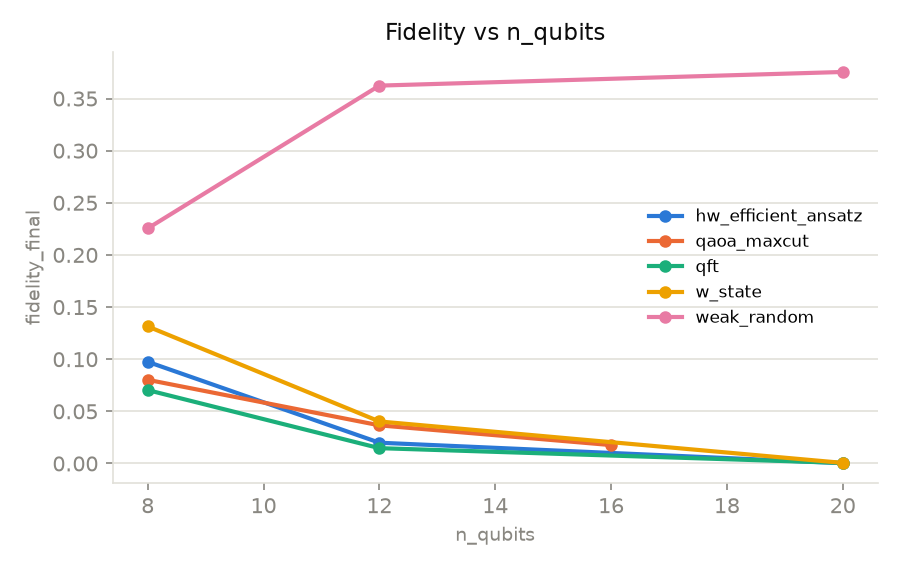
\includegraphics[width=0.75\linewidth]{figures/scaling_fidelity.png}
  \caption{Mean \texttt{fidelity\_final} vs.\ qubit count, per circuit
    family, pooled across the three per-block optimizers of the
    225-run core baseline (Section~\ref{sec:case-study:algorithms}).
    Four of five families decline toward the metric's near-zero floor
    as $n$ grows; \texttt{weak\_random} is the exception. A single-scale
    evaluation of any one family in isolation -- the norm in the
    QIEA-MOO literature surveyed above -- would surface only one point
    on this plot.}
  \label{fig:scaling-fidelity}
\end{figure}

More fundamentally, the
Pareto-dominance relation every classical MOEA baseline in
Section~\ref{sec:background:moea} and every NSGA-II-hybridized QIEA-MOO
method in Section~\ref{sec:taxonomy:hybridization} relies on has itself
only recently been shown to have a structural weakness --
\citet{zheng2025weakparetoboundary}'s ``weak Pareto boundary'' result --
that postdates nearly all of the surveyed QIEA-MOO literature and so
could not have been accounted for by it. Scalability claims in this field, in short, rest on baselines and
dominance relations whose own limits are still being discovered, on top
of application-side evaluations that rarely test more than one problem
scale to begin with.
